\documentclass{scrartcl}			% defines the kind of document you want to produce

% Include different packages:
\usepackage[utf8]{inputenc}
\usepackage[T1]{fontenc}
\usepackage{lmodern}
\usepackage[english]{babel}
\usepackage{amsmath}
\usepackage{graphicx}           	% include graphics
\usepackage{caption}	
\usepackage{subcaption}	 
\usepackage{hyperref}
\usepackage{epstopdf}
\usepackage{siunitx}
\usepackage{float}

\title{Neuroprothetics Exercise 5\\Multicompartment Model}
\author{ Laura Bielenberg }
\date{08. Juni 2019}

\begin{document} 					% Document begins here

\maketitle

\section{Create a Multicompartment Model}

Change the point neuron model from the last exercise to a multicompartment model consisting of $n = 100$ Compartments. Modify the functions from the last exercise to work with arrays of dimension $n × 1$ instead of scalar values. Implement the cable equation inside \texttt{hh\_current}, have a look at the slides provided in moodle for more information. Use the forward Euler method to solve the arising system of differential equations. The parameters are given in the Appendix.\\
\newline
The code has been written using \textbf{python 3}. Most of the implementation could be done by reusing functions from the last exercises, since they were already able to work with vectorized inputs. For more details see \texttt{Neuroprosthetics/multicompartment\_model.py} and \texttt{exercise\_5.py}.\\
\newline
New parameters are the connection matrix $\mathbf{C}$ as well as the resistance along the axon $R_a$. The former one has the form
\begin{equation}
\mathbf{C} = \begin{pmatrix}
	-1& 1 &&&0\\
	1& -2& 1\\
	&\ddots&\ddots&\ddots\\
	&& 1& -2& 1\\
	0&&&1&-1
	\end{pmatrix}
\end{equation}
while the latter one is calculated as
\begin{equation}\label{eqn:ra}
R_a = \frac{\rho_{axon}  d_l}{\pi  r_{axon}^2}\, .
\end{equation}

\newpage
\section{Experiments}
Run $\SI{100}{\milli\second}$ long simulations ($\Delta t = \SI{25}{\micro\ampere}$) at $\SI{6.3}{\celsius}$ with the following settings.
\subsection{Stimulation at first compartment}
The axon has been stimulated at the first compartment with a rectangular 5ms long pulse and an amplitude of \SI{10}{\micro\ampere}. Figure\ref{fig:comp1} shows how the action potential propagates along the axon.

\begin{figure}[H]
\centering
\includegraphics[width=\linewidth]{imgs/compartment_model0.eps} 
    \caption{Propagation of the action potential for stimulation at compartment 1.} 
    \label{fig:comp1} 
\end{figure}

\subsection{Simultaneus stimulation at compartments 20 and 80}
In figure~\ref{fig:comp2} the axon is stimulated with the same pulse as above but at compartments 20 and 80 simultaneously.\\ Looking at the figure it can be seen, that the action potential propagates along both the directions of the axon starting from each of the stimulation points.

\begin{figure}[H]
\centering
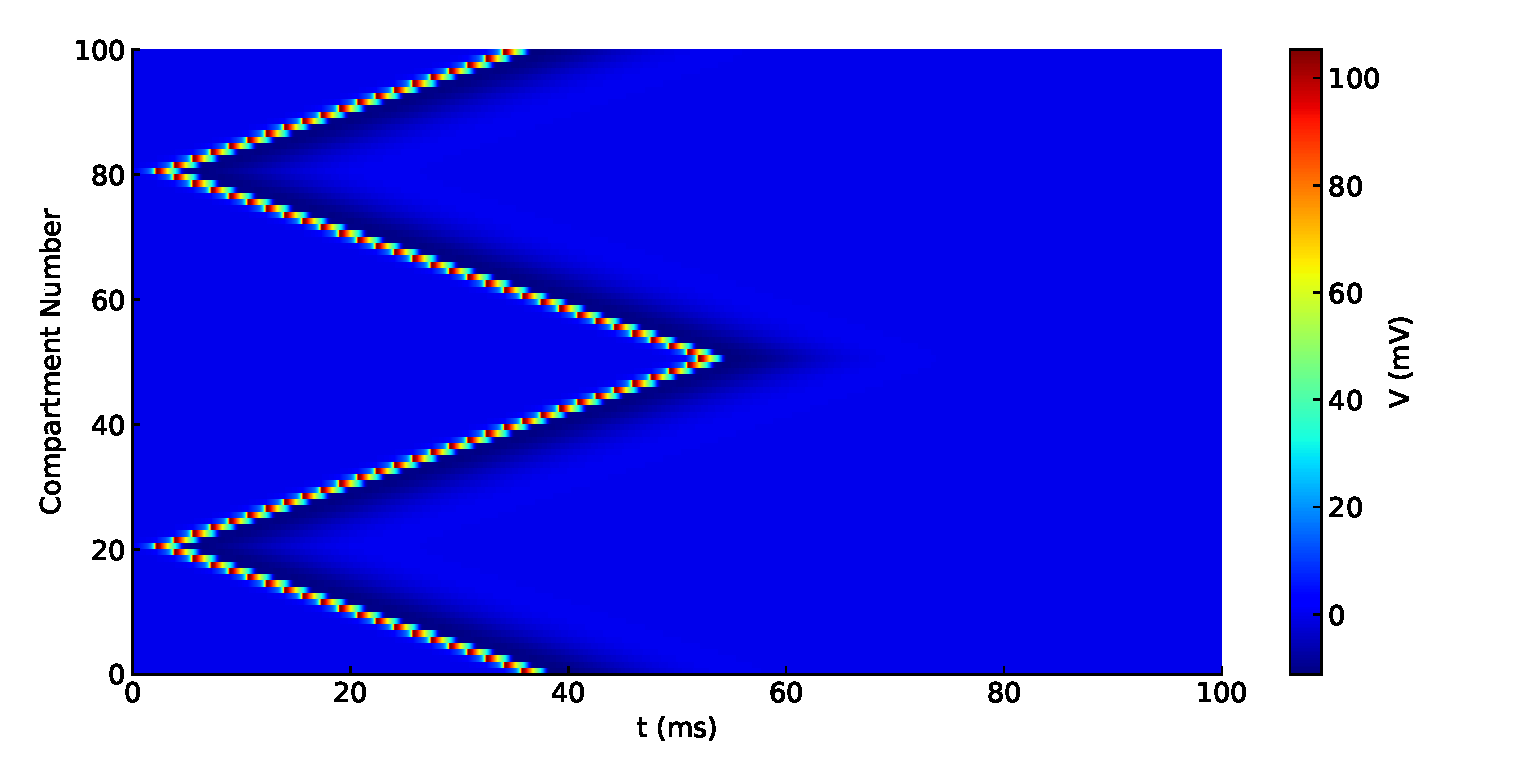
\includegraphics[width=\linewidth]{imgs/compartment_model2080.eps} 
    \caption{Propagation of the action potential for stimulation at compartment 1.} 
    \label{fig:comp2} 
\end{figure}

\subsection{Parameter exploration}
Explore the different parameters of the model, find out which affect the speed of action potential propagation and explain your findings.\\
\newline
\textbf{Answer:}\\
In the underlying differential equation of the multi compartment model
\begin{equation}\label{eqn:ode}
	\frac{d}{dt} V = \frac{1}{C_m} (-i_{HH}(V, t) + i_{stim}(t)) + \frac{1}{C_m R_a} \mathbf{C} V \, ,
\end{equation}
the term 
\begin{equation}
\tau = \frac{1}{C_m R_a}
\end{equation}
 represents the systems timeconstant. Thus changes in the membrane Capacity as well as changes of the overall axon resistance change the speed in which the action potential travels along the axon. This can also be seen in figure~\ref{fig:comp3}, where the action potential propagation is shown for different settings of $C_m$ and $R_a$. The larger $C_m$ and $R_a$ get, the longer it takes for the signal to be propagated.\\
Considering the relationship between axon resistance, axon length and axon radius given in equation\ref{eqn:ra} it can be concluded that: \\The longer the axon and the smaller its radius,  the higher its resistance $R_a$ and thus the slower its signal propagation.
\begin{figure}[H]
\centering
\includegraphics[width=\linewidth]{imgs/different_settings_Ra_Cm.eps} 
    \caption{Qualitative propagation of action potentials for different settings of $R_a$ and $C_m$ after stimulation at compartment 1.} 
    \label{fig:comp3} 
\end{figure}


\end{document}
